\documentclass[letter,10pt,openany,oneside]{book}
\usepackage[utf8]{inputenc}
\usepackage[spanish, activeacute]{babel}
\usepackage{amsmath}
\usepackage{tikz}
\usepackage{forest}
\usepackage{float}
\usepackage[margin=2cm]{geometry}
\usepackage{multicol}
\usepackage{csquotes}
\usepackage{nth}
\usepackage{graphicx}
\usepackage{minted}
\usepackage{chessboard}
\usepackage{xskak}
\usepackage{capt-of}
\usepackage{fancyhdr}
\usepackage[explicit]{titlesec}
%\usepackage{showframe}

%\titlespacing\section{0pt}{0pt plus 1pt minus 1pt}{0pt plus 2pt minus 2pt}
%\titlespacing\subsection{0pt}{0pt plus 1pt minus 1pt}{0pt plus 2pt minus 2pt}
%\titlespacing\subsubsection{0pt}{12pt plus 4pt minus 2pt}{0pt plus 2pt minus 2pt}






\makeatletter
\let\@chapterimage\relax
\newcommand\chapterimage[1]{%
  \if\relax\detokenize{#1}\relax
  \else
    \gdef\@chapterimage{\smash{\includegraphics[height=2.4cm,keepaspectratio]{#1}}}
  \fi
}

\makeatletter
\let\@chapterimageb\relax
\newcommand\chapterimageb[1]{%
  \if\relax\detokenize{#1}\relax
  \else
    \gdef\@chapterimageb{\smash{\includegraphics[height=2.5cm,keepaspectratio]{#1}}}
  \fi
}

\titleformat{\chapter}[display]
  {\normalfont\huge\bfseries}
  {}
  {0pt}
  {\parbox[t]{.4\textwidth}{\chaptertitlename\ \thechapter}\hfill
    \parbox[t]{.4\textwidth}{\@chapterimage}\\[20pt]%
    \center\Huge#1
  }
  
\titleformat{name=\chapter,numberless}[display]
  {}
  {}
  {0pt}
  { \parbox[t]{\textwidth}{\@chapterimageb}\hfill
    \parbox[t]{\textwidth}{\@chapterimage}\\[10pt]%
    \normalfont \centering \LARGE \bf #1
  }
  [
    \vspace{-1cm}
  ]
  
\titlespacing*{\chapter}{0pt}{0pt}{40pt}

\newcommand\nochapterimage{
  \let\@chapterimage\relax
}
\makeatother

%\setlength{\parskip}{5mm}
\pagestyle{fancy}

\fancyfoot[R]{\thepage}
\renewcommand{\headrulewidth}{0pt}
\renewcommand{\footrulewidth}{1pt}
\fancyfoot[C]{}
\newcommand{\TheAuthor}{}
\newcommand{\Author}[1]{\renewcommand{\TheAuthor}{#1}}
\lfoot{\TheAuthor}

\fancypagestyle{plain}{

\renewcommand{\headrulewidth}{0pt}
\fancyfoot[R]{\thepage}
\fancyfoot[C]{}
\lfoot{\TheAuthor}}

%%%%%%%%%%%%%%%%%%%%%%%%%%%%%% User specified LaTeX commands.

\begin{document}


\chapterimage{images/dsc}
\chapterimageb{images/logo}

%\chapter*{}
\vspace{-1cm}
\begin{center}
    \Huge \bf Concurso de la XV Semana de MAC
\end{center}

\bigskip

\subsection*{Indicaciones:}

\begin{itemize}

	\item La entrada del programa se debe leer de la entrada estándar \texttt{stdin}.
    
    \item La salida de programa se debe imprimir a la salida estándar \texttt{stdout}.
    
    \item Trata de usar métodos de lectura y escritura rápida para tus problemas, puesto que existen algunos problemas cuyas entradas pueden ser muy grandes.
    
    \item Una unidad de tiempo de tiempo para cada lenguaje son: \texttt{C} $\rightarrow$ 1 segundo, \texttt{C++} $\rightarrow$ 1 segundo, \texttt{C++14} $\rightarrow$ 1 segundo, \texttt{Java7} $\rightarrow$ 2 segundos, \texttt{Java8} $\rightarrow$ 2 segundos, \texttt{Python2} $\rightarrow$ 5 segundos y \texttt{Python3} $\rightarrow$ 5 segundos. De tal manera que si un problema dice 2u, en \texttt{Java7} tendrá un tiempo límite de 4 segundos.
   	
    \item No imprimir cadenas como: ``Dame la entrada'', ``La salida es:''
    \begin{minted}{cpp}
		printf("Dame la entrada:");/*Esto no se debe hacer*/
	\end{minted}
    
    \item No usar bibliotecas no estándar
  	
    Ejemplo:
    
    \begin{minted}{cpp}
#include <conio.h> /*Esta librería no es estándar*/

int main()
{
     system("pause");//No usar esto
     getch();//Ni esto
    
     return 0;
}
    \end{minted}
    
    \item Los problemas deberán llamarse como se indica en ``Código Fuente'', por ejemplo, para el primer problema si está hecho en Java será: \texttt{alreves.java}.
    
    \item Recuerda que está prohibido accesar a cualquier recurso de internet que no sean los señalados explícitamente el día del concurso.
    
    \item El usar cualquier dispositivo electrónico ajeno al concurso durante el transcurso del mismo es motivo de descalificación.
        
\end{itemize}

\subsection*{Mensaje al competidor}
Todos los problemas presentados aquí son originales e inéditos, elaborados por el Grupo de Algoritmia Avanzada y Programación Competitiva de la Facultad. Agradecemos a la Jefatura de MAC por el apoyo prestado para la elaboración de este concurso, así como, al Departamento de Servicios de Cómputo del CeDeTec por su constante presencia, apoyo, y patrocinio. 

Esperamos que se diviertan resolviendo estos problema.

Si les gustó el reto, no duden en preguntarnos cómo unirse al grupo y asistir a la sesión donde les enseñaremos a resolver todos los problemas del concurso.

\bigskip

\begin{center}
    \Large \it Happy Coding!
\end{center}


\thispagestyle{empty}

\newpage
\chapter*{Problema A - ¡Arriba, Papalotes, Arriba!}

Queremos hacer papalotes triangulares y tú nos
ayudarás. Para eso tenemos 5 varas de madera que nos
servirán a darle forma al papalote como nosotros 
lo deseamos. 

La siguiente figura nos ayudará a ilustrarte el tipo
de papalotes que pretendemos hacer.

\begin{center}
    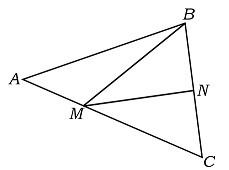
\includegraphics{images/Triangulo.jpg}
\end{center}

Tres de las varas con las que contamos ($AB$, $BC$ y 
$CA$) las usaremos para delimitar la figura del 
triángulo; una más se colocará a partir del vértice 
$B$ hacia algún punto $M$ del lado opuesto; la 
última irá del punto $M$ hacia algún punto $N$ sobre
el segmento $BC$.

Necesitamos cortar el material que va en los 
triángulos ABM, BMN y CMN,
y debemos ser muy cuidadosos para crear bellos 
papalotes. Obtener el área de los mencionados 
triángulos será tu trabajo.

¡Ah! Una cosa más. Te daré un dato que tal vez pueda
serte útil. El área de un triángulo se puede obtener
con la siguiente fórmula:
$$A = \sqrt{S \cdot (S-a) \cdot (S-b) \cdot (S-c)}$$
donde $a, b$ y $c$ son los lados del triángulo y $S$ es
su semiperímetro.




\subsection*{Entrada}
La primera línea de la entrada contendrá un número $T$, 
el número de casos. Luego vendrán $T$ líneas -una para
cada caso; cada una estará compuesta por 5 números 
reales positivos separados por un espacio, que 
representarán la longitud de los segmentos $AB$, $BC$,
$CA$, $MC$ y $NC$, en ese orden.




\subsection*{Salida}
Imprime las áreas de los tres triángulos en orden 
ascendente, cada área en una línea distinta. Repite
el proceso para cada caso.

Tendrás un margen de error $10^{-5}$.



\subsection*{Límites de los conjuntos de datos}

\begin{itemize}
    \item Grande: $ \;\, 1 \leq T \leq 10^{3}$, 
    $0 < AB, BC, CA, MC, NC \leq 100$ $\quad \;\,$ $100$ puntos.
\end{itemize}



\begin{multicols}{2}

\subsection*{Entrada Ejemplo}

\begin{verbatim}
1
13 4 15 6 1
\end{verbatim}

\columnbreak

\subsection*{Salida Ejemplo}

\begin{verbatim}
2.4
7.2
14.4
\end{verbatim}

\end{multicols}

\newpage
\chapter*{Problema B - Buenos Amigos}
%ÁÉÍÓÚÑáéíóúñ  ``  ''
¿Te has dado cuenta que en el salón de clases las personas se juntan por grupitos?

A Joaquina le gusta esa idea, ya que no quiere ser amiga de todos, y se pregunta lo siguiente: ¿Cuál es la máxima cantidad de amistades que puede haber en un salón de $n$ alumnos de tal manera que nadie sea amigo de todos los demás?

Toma en cuenta que si la persona $a$ es amiga de $b$, entonces $a$ es amiga de todos los amigos de $b$ y viceversa.

\subsection*{Entrada}
La primera línea contendrá un número $T$, el número de 
casos de entrada. Posteriormente vendrán $T$ líneas, cada 
una con un entero positivo $n$, el número de personas en el salón.



\subsection*{Salida}
Para cada caso, imprime en una línea distinta la máxima cantidad de amistades que se pueden formar.

\subsection*{Límites de los conjuntos de datos}

\begin{itemize}
    \item Pequeño: $ 1 \leq T \leq 10^2 $, $ 1 \leq n
    \leq 10^2$   $\quad \;\;\;\;\;$ $30$ puntos.
    \item Mediano: $ 1 \leq T \leq 10^3 $, $ 1 \leq n
    \leq 10^4$   $\quad \;\;\;\;\;$ $30$ puntos.
    \item Grande: $ 1 \leq T \leq 10^5 $, $ 1 \leq n
    \leq 10^8$   $\quad \;\; \;\;\;\;\;$ $40$ puntos.
\end{itemize}



\begin{multicols}{2}

\subsection*{Entrada Ejemplo}

\begin{verbatim}
2
3
2
\end{verbatim}

\columnbreak

\subsection*{Salida Ejemplo}

\begin{verbatim}
1
0
\end{verbatim}

\end{multicols}

\newpage
\chapter*{Problema C - Cuando una Hámster Quiere Jugar}

A mi hámster le encanta jugar. Hoy decidió salir al
patio a escavar hoyos para matar el aburrimiento. Para 
su comodidad decidí trazar líneas en el patio de tal 
forma que éste fuera una cuadrícula, y en cada uno de 
los cuadros haya una piedra en algún punto que no le 
permitirá a la roedora hacer un hoyo más profundo.

Mi hámster comienza en el cuadro que más le guste en
ese momento y saca toda su tierra hasta encontrar la
piedra. Luego, se mueve a alguno de los cuadros con los
que comparte al menos un vértice y escarva hasta que se
encuentre con la piedra de ese cuadro, o bien, hasta que
alcance la misma profundidad con la que quedó el cuadro 
anterior, lo que suceda \textit{primero}. La inteligente
roedora continúa con este proceso hasta que se encuentre
con una piedra a nivel del suelo, es decir, a profundidad
0.

Considerando que la hámster puede moverse y regresar a
dónde ella desee y que puede moverse de manera 
horizontal, vertical y diagonal en la dirección que 
quiera, ¿cuál es la máxima cantidad de tierra que puede
sacar?
$$ $$
\textbf{Nota:} Mi hámster tiene un asistente que retira
la tierra en cuanto hace un hoyo, así que no tienes que 
preocuparte por pensar qué sucederá una vez que la 
tierra esté fuera del cuadro.




\subsection*{Entrada}
La primera línea estará compuesta por dos números 
naturales $m$ y $n$, que indicarán el tamaño de la 
cuadrícula de la que dispone mi hámster. Luego, se te
dará una matriz $M$ de enteros no negativos de $m \times 
n$, en la que te indicaremos cuál es la profundidad de la
piedra en ``unidades hamsterunas" (las coordenadas de la
matriz empiezan en 1). Finalmente, encontrarás una línea
compuesta por dos enteros $s_i$ y $s_j$, las coordenadas 
del punto en el que el animalillo decidió comenzar.



\subsection*{Salida}
Imprime, en unidades hamsterunas, la máxima cantidad de
tierra que mi mascota podrá sacar.



\subsection*{Límites de los conjuntos de datos}

\begin{itemize}
    \item Pequeño: $1 \leq m, n \leq 50$, $0 \leq m_{ij} 
    \leq 100$, $1 \leq s_i \leq m$, $1 \leq s_j \leq n$
    $\quad \;\;\;\;\;\;\;$ $35$ puntos.
    \item Mediano: $1 \leq m, n \leq 50$, $0 \leq m_{ij} 
    \leq 10^9$, $1 \leq s_i \leq m$, $1 \leq s_j \leq n$
    $\quad \;\;\;\;\;\;\;$ $20$ puntos.
    \item Grande: $1 \leq m, n \leq 500$, $0 \leq m_{ij} 
    \leq 10^{10}$, $1 \leq s_i \leq m$, $1 \leq s_j \leq 
    n$    $\quad \;\;\;\;\;$ $45$ puntos.
\end{itemize}



\begin{multicols}{2}

\subsection*{Entrada Ejemplo}

\begin{verbatim}
3 3
5 0 5
1 2 1
0 0 5
2 2
\end{verbatim}

\columnbreak

\subsection*{Salida Ejemplo}

\begin{verbatim}
10
\end{verbatim}

\end{multicols}

%%%%%%%%%%%%%%%

\begin{multicols}{2}

\subsection*{Entrada Ejemplo}

\begin{verbatim}
2 5
2 3 4 0 1000
3 2 3 0 1000
2 1
\end{verbatim}

\columnbreak

\subsection*{Salida Ejemplo}

\begin{verbatim}
16
\end{verbatim}

\end{multicols}

\newpage
\chapter*{Problema D - Déjalo a la Suerte}
%ÁÉÍÓÚÑáéíóúñ  ``  ''
Vamos a jugar un juego de azar.

Si quieres participar, debes adquirir una papeleta en
la que podrás seleccionar (o no) los números que 
desees entre $1$ y $n$ y registrarlos. Puedes selccionar
la cantidad de números que quieras, siempre y cuando
sea más de uno y menos de $n-1$.

Como suele suceder con este tipo de juegos, habrá un
anfitrión que sacará de una urna una papeleta ganadora,
y listo, ganará la persona que tenga la papeleta con 
los mismos números seleccionados que los del anfitrión.

Para ganar, únicamente es necesaria la existencia de 
los mismos números del anfitrión, sin importar el 
orden.

Si podemos asegurar que no hay dos papeletas que sean
registradas iguales, ¿cuál es la probabilidad
de que ganes si adquieres $k$ papeletas?

Como la probabilidad puede ser muy muy pequeña, 
necesitamos que multipliques tu respuesta por $10^{15}$.
Tendrás un margen de error de $10^{-5}$.




\subsection*{Entrada}
La primera línea contendrá un entero positivo $T$ (el 
número de casos a leer). Luego vendrán $T$ líneas, cada
una compuesta por dos enteros positivos separados por 
un espacio: $n$ y $k$, en ese orden.




\subsection*{Salida}
Para cada caso imprime en una línea distinta la 
probabilidad que tengas de ganar.                   




\subsection*{Límites de los conjuntos de datos}

\begin{itemize}
    \item Pequeño: $ 1 \leq T \leq 100 $, $4 \leq n 
    \leq 10$, $k < n$ $\quad \;\;\;$ $30$ puntos.
    \item Mediano: $ 1 \leq T \leq 100 $, $4 \leq n
    \leq 20$, $k < n$   $\quad \;\;\;$ $20$ puntos.
    \item Grande: $ \;\, 1 \leq T \leq 100$, $ 1 
    \leq n \leq 60 $, $k < n$ $\quad \;\;\;$ $50$ puntos.
\end{itemize}



\begin{multicols}{2}

\subsection*{Entrada Ejemplo}

\begin{verbatim}
3
4 1
10 3
18 6
\end{verbatim}

\columnbreak

\subsection*{Salida Ejemplo}

\begin{verbatim}
166666666666666.66667
2994011976047.90419
22891501911.44041
\end{verbatim}

\end{multicols}

\newpage
\chapter*{Problema E - Están entre Nosotros}
%ÁÉÍÓÚÑáéíóúñ  ``  ''
Antes de poder entrar a la sala para participar en el concurso de programación, a todos los concursantes se les hizo formarse en una línea, y se les asignó un número de mesa distinto (no necesariamente en forma ascendente o descendente), mismos que componen un arreglo de enteros.

A mi hámster (que es una genio) le gustan mucho las series de televisión, y una de sus favoritas le dio la idea de crear este problema. Ella elige una secuencia mágica, llamada ``la secuencia de los Elegidos", y se pregunta si ésta es subsecuencia del arreglo que forman las personas en la fila.



%A mi hámster (que es una genio) le gustan mucho las secuencias númericas, y se pregunta si la secuencia de ``los Elegidos'' es una subsecuencia de la secuencia formada por las personas en la fila.

%La secuencia de ``los Elegidos'' es una secuencia que mi hermosísima hámster vio en una de sus series de televisión favoritas.





\subsection*{Entrada}

La primera línea de entrada es un número $T$ (el número de
casos de prueba). Siguen los $T$ casos: cada uno está
compuesto por tres renglones, el primero de ellos tiene dos numeros: $S$ y   $E$, el número de concursantes y el tamaño de la secuencia de ``los Elegidos'', respectivamente; en el segundo renglón vendrá la secuencia formada por los concursantes y en el tercero la de ``los Elegidos".




\subsection*{Salida}

Para cada caso de entrada deberás imprimir en una línea distinta ``Estan entre nosotros'' si la secuencia de ``los Elegidos'' es subsecuencia de la secuencia formada por los concursantes o ``You always knew'' en caso contrario (sin acento y sin comillas).

\subsection*{Límites de los conjuntos de datos}

\begin{itemize}
    \item Pequeño: $ 1 \leq T \leq 1000 $, $ 1 \leq S, E
    \leq 100$, $1 \leq s_i, e_j \leq 100$   $\quad \;\;\;\;\;$ $40$ puntos.
    \item Mediano: $ 1 \leq T \leq 100 $, $ 1 \leq S, E
    \leq 10^{3}$, $1 \leq s_i, e_j \leq 10^9$   $\quad \;\;\; \quad$ $30$ puntos.
    \item Grande: $ \;\, 1 \leq T \leq 20$, $ 1 
    \leq S, E \leq 10^{5} $, $1 \leq s_i, e_j \leq 10^{15}$ $\quad \;\;\;\;\; \quad$ $30$ puntos.
\end{itemize}




\begin{multicols}{2}

\subsection*{Entrada Ejemplo}

\begin{verbatim}
2
7 6
4 8 15 12 16 23 42
4 8 15 16 23 42
3 3
1 2 3
3 2 1
\end{verbatim}

\columnbreak


\subsection*{Salida Ejemplo}

\begin{verbatim}
Estan entre nosotros
You always knew
\end{verbatim}

\end{multicols}


\end{document}